%----------------------------------------------------------------------------------------
%	PACKAGES AND OTHER DOCUMENT CONFIGURATIONS
%----------------------------------------------------------------------------------------
 
\documentclass[12pt]{article}
    \usepackage{graphicx} %Needed for logos
    \usepackage{tikz}
    \usetikzlibrary{matrix,calc} 
    \usepackage{fancyhdr}
    \pagestyle{fancy}
    \fancyhead[L]{Left}
    \fancyhead[R]{Right} 
    \fancyhead[C]{Center}
    \usepackage{lastpage}
    \usepackage{float}
    \usepackage{amsmath}
    \usepackage{enumerate,letltxmacro}
    \LetLtxMacro\itemold\item
    \renewcommand{\item}{\itemindent1cm\itemold}
    \usepackage{enumitem} 
    \usepackage{verbatim} 
    \usepackage[english]{babel}
    \usepackage{blindtext}
    \usepackage{varwidth}
    \setlength\parindent{24pt}
    \usepackage{booktabs} 
    \usepackage{tabularx}
    \newcolumntype{C}{>{\centering\arraybackslash}X}
    \usepackage{bm}  
    \usepackage[object=vectorian]{pgfornament} 
    \usepackage{tikzpagenodes}
    \usepackage{lipsum}
    \usepackage{booktabs,pdflscape,adjustbox} 
    \usepackage{abstract}
    \usepackage{setspace}
    \usepackage{ragged2e}
    \usepackage{listings}
    \usepackage{color, xcolor}
    \usepackage{fancybox}
    \usepackage{hyperref}
    \usepackage{fontawesome}
    \usepackage{subcaption}
    \usetikzlibrary{arrows,positioning,automata}
    \usepackage{tkz-graph}
    \usepackage{amsfonts}
    
    \usepackage[margin=0.95in]{geometry}
    
    %----------------------------------------------------------------------------------------
    %	TITLE PAGE
    %----------------------------------------------------------------------------------------
    
    \newcommand*{\titleGP}{\begingroup % Create the command for including the title page in the document
    \centering % Center all text
    \vspace*{\baselineskip} % White space at the top of the page
    \vspace*{-1.0cm}
    \centerline{\rule{17cm}{1.6pt}}\vspace*{-\baselineskip}\vspace*{2pt} % Thick horizontal line
    \centerline{\rule{17cm}{0.4pt}}\ \\[\baselineskip] % Thin horizontal line
    
    {\LARGE 332:573 -- Data Structures \& Algorithms \\ \Large Project Report \\ \vspace*{0.3cm} \large Improvements to Polynomial Multiplication Through Fast Fourier Transforms\vspace*{0.2cm}\small \\By David Lambropoulos, Demetrios Lambropoulos}
    % Title 
    
    \centerline{\rule{17cm}{0.4pt}}\vspace*{-\baselineskip}\vspace{3.2pt} % Thin horizontal line
    \centerline{\rule{17cm}{1.6pt}}\ \\[\baselineskip] % Thick horizontal line
    \vspace*{-0.35cm}Professor Shantenu Jha\par
    May $\text{6}^\text{th}$, 2018\par
    \vfill 
    \vspace*{10.3cm}
    \centerline{
\includegraphics[scale=0.5]{images/rulogo}} 
    \textit{Rutgers University}\par
    \textit{School of Engineering}\par
    
    \vspace*{2\baselineskip} % Whitespace between location/year and editors
    
    \vfill % Whitespace between editor names and publisher logo
    
        
    \endgroup}
    
    %----------------------------------------------------------------------------------------
    %   CENTERED BOX
    %----------------------------------------------------------------------------------------
    \makeatletter
    \newenvironment{CenteredBox}{% 
    \begin{Sbox}}{% Save the content in a box
    \end{Sbox}\centerline{\parbox{\wd\@Sbox}{\TheSbox}}}% And output it centered
    \makeatother
        
        
    %----------------------------------------------------------------------------------------
    %   LSTLISTING CODE DEFINITION
    %----------------------------------------------------------------------------------------
    \definecolor{codegreen}{rgb}{0,0.6,0}
    \definecolor{codegray}{rgb}{0.5,0.5,0.5}
    \definecolor{codepurple}{rgb}{0.58,0,0.82}
    \definecolor{backcolour}{rgb}{0.95,0.95,0.92}
        
    \lstdefinestyle{mystyle}{
        backgroundcolor=\color{backcolour},   
        commentstyle=\color{codegreen},
        keywordstyle=\color{magenta},
        numberstyle=\tiny\color{codegray},
        stringstyle=\color{codepurple},
        basicstyle=\footnotesize,
        breakatwhitespace=false,         
        breaklines=true,                 
        captionpos=b,                    
        keepspaces=true,                 
        numbers=left,                    
        numbersep=5pt,                  
        showspaces=false,                
        showstringspaces=false,
        showtabs=false,                  
        tabsize=4
    }
    
    %----------------------------------------------------------------------------------------
    %	BUILD HEADER
    %----------------------------------------------------------------------------------------
    
    % Length to control the \fancyheadoffset and the calculation of \headline
    % simultaneously
    \newlength\FHoffset
    \setlength\FHoffset{1cm}
    
    \addtolength\headwidth{2\FHoffset}
    
    \fancyheadoffset{\FHoffset}
    
    % these lengths will control the headrule trimming to the left and right  
    \newlength\FHleft
    \newlength\FHright
    
    % here the trimmings are controlled by the user
    \setlength\FHleft{1cm} 
    \setlength\FHright{0cm}
    
    % The new definition of headrule that will take into acount the trimming(s)
    \newbox\FHline
    \setbox\FHline=\hbox{\hsize=\paperwidth%
        \hspace*{\FHleft}%
        \rule{\dimexpr\headwidth-\FHleft-\FHright\relax}{\headrulewidth}\hspace*{\FHright}%
    }
    \renewcommand\headrule{} 
    
    
    %----------------------------------------------------------------------------------------
    %	BODY OF DOCUMENT
    %----------------------------------------------------------------------------------------
    
    \begin{document}    
        \pagestyle{empty} % Removes page numbers 
        \onecolumn
        \titleGP % This command includes the title page
        \newpage
        \renewcommand*\contentsname{Contents}
        \tableofcontents
        \newpage 
        
        \setcounter{page}{1}
        \pagestyle{fancy}
        \lhead{David, Demetrios\\} 
        \chead{NetID: dal220, dpl60\\ \myrule} 
        \rhead{332:573 -- Algorithms\\ \myrule}
        \lfoot{\vspace*{-0.1cm}\myrule \\ \vspace*{0.1cm}Project Report -- FFT Improvements to Polynomial Multiplication}
        \cfoot{}
        \rfoot{\vspace*{-0.1cm}\myrule \\\vspace*{0.1cm}Page - \thepage{} }
        
        \newcommand\myrule{%
            \leavevmode\cleaders\hbox{\raisebox{-2.5pt}{\pgfornament[width=0.2\textwidth]{88}}}\hfill\kern0pt}

        
        \section{Introduction/Motivation}
        \indent\par{Polynomials are expressions built up of a combination of constants $c$ and symbols called variables. Polynomials with a single indeterminate x can always be written in the form }
        $$a_nx^n + a_{n-1}x^{n-1} + ... + a_2x^2 + a_1x + a_0$$
        \par{where $a_0,...,a_n$ are constants and x is the indeterminate variable. Polynomials can also be expressed in the following canonical form}
        $$ \sum_{k=0}^{n}a_kx^k $$
        \indent\par{Each term in a polynomial is product of some constant called the coefficient of the term and indeterminate raised to a nonnegative integer power n (i.e.$n\in\mathbb{Z}^+$). Polynomials are used in many fields to represent problems or model behavior such as Chemistry, Physics, Economics, Social Scientists, Calculus, Numerical Analysis, etc.}
        \indent\par{Addition and subtraction of polynomials is easy to implement costing only $O(N)$ time. However, the way polynomials are multiplied is through a method called First, Outer, Inner, Last (FOIL) as can be seen below in Figure \ref{fig:foil}. The issue with the FOIL method is that it requires too many operations to perform multiplications, especially for large polynomials. Usually real world problems will be modeled with polynomials of 10000+ terms.}
        \begin{figure}[H]
        	\centerline{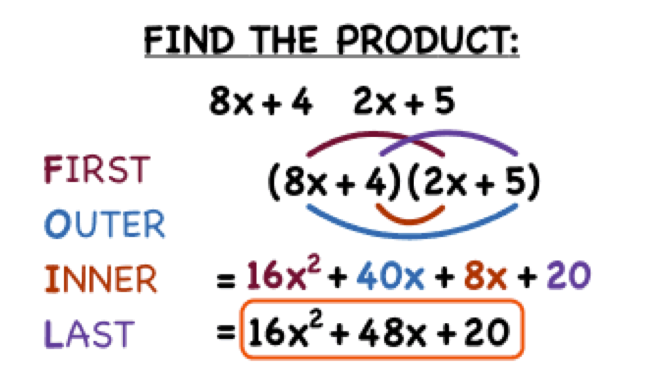
\includegraphics[scale=0.5]{images/FOIL}}
        	\caption{Demonstration of FOIL method}
        	\label{fig:foil}
        \end{figure}
    	\indent\par{The main scientific motivation behind improving the speed in which we multiple polynomials is that solving large polynomials by hand is tedious and error prone. As discussed previous solving large polynomial multiplications through quadratic algorithms (i.e. FOIL) would cost more time than any person might have. A way that can fix this costly calculation is to implement recursion which uses the divide and conquer method.}
    	  
        \section{Algorithms/Theory}
        \indent\par{Given a polynomial $A(x)$ of length $m$ and a secondary polynomial $B(x)$ of length $n$ then the resultant product would have a length of $m+n-1$. As mentioned before, a polynomial can be represented as a sum of terms consisting of constant coefficients and indeterminate variables as follows: }
        $$A(x) = \sum_{k=0}^{n}a_kx^k = a_nx^n + a_{n-1}x^{n-2} + ... + a_1x + a_0$$
        \indent\par{When representing a polynomial in code, we can represent as an array of coefficients in reverse order ($a = [a_0,a_1,...,a_{n-1}]$). The main advantage to representing this as such allows us to reference coefficients via array indexes. }
        \indent\par{We can start analyzing the FOIL method more formally as follows. Given a polynomial:}
        $$ A(x)=\sum_{j=0}^{n-1}a_jx^j $$
        \par{and a polynomial}
        $$ B(x) =\sum_{j=0}^{n-1} b_jx^j $$
        \par{The polynomial multiplication in brute force would be given by }
        $$ C(x)=\sum_{j=0}^{n-1}\sum_{k=0}^{n-1}a_jb_kx^{j+k} $$
        \par{resulting in a runtime of $O(n^2)$}
        \indent\par{The Fast Fourier Transform (FFT) is an improvement on the Discrete Fourier Transform (DFT) algorithm and has been recognized as on the best algorithms of the $20^{th}$ century\cite{dongarra2000guest}. The DFT is represented as: }
        $$X(n)=\sum_{k=0}^{N-1}x[k]e^{-j(2\pi kn/N)}$$
        \indent\par{The DFT algorithm can easily be seen that there are $N$ additions by $N$ multiplications resulting in a runtime of $O(N^2)$. The FFT factors the DFT matrix into sparse factors resulting in a runtime of $O(N log N)$.}
        \section{Experimental Setup}
        \indent\par{The datasets that were used in the program were randomly generated with $generateDatasets.py$ file. This generated datasets of sizes 1, 2, 4, 8, 16, 32, 64, 128, 256, 512, 1024, 2048, and 4096. The experiment was run on Windows (Processor Intel (R) Core (TM) i7-3630QM CPU @ 2.40GHz, 2401 Mhz, 4 Cores(s), 8 Logical Processor, 8GB RAM) running Windows 10. The program was implemented with Python 3.6.}
        \section{Results and Analysis} 
        \indent\par{Too better see the competition of the Brute Force algorithm and the FFT algorithm we analyzed the results for polynomials less than degree 40. The output can be seen in Figures \ref{fig:assignZoom} and \ref{fig:compZoom}. The zoomed in FFT has less assignments and comparisons in the long run. However, there exists a small period where for small polynomials brute force outperforms the FFT. Next, looking at polynomials up to 8192 terms shows that the FFT almost disappears in comparison to the brute force algorithm. This can be seen in Figures \ref{fig:assign8192} and \ref{fig:comp8192}.}
        \begin{figure}[H]
            \centerline{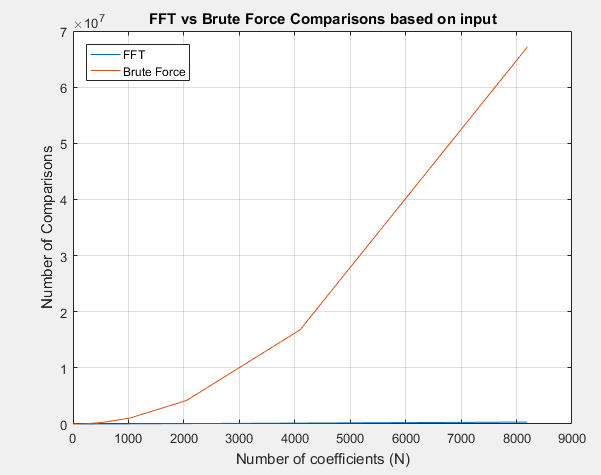
\includegraphics[scale=0.5]{images/BruteVSFFT_8192_Comparisons}}
            \caption{Number of Comparisons. FFT vs Brute Force.}
            \label{fig:comp8192} 
        \end{figure}
        \begin{figure}[H]
            \centerline{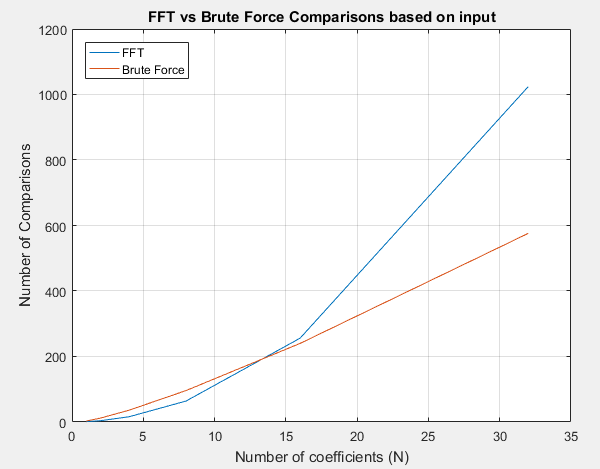
\includegraphics[scale=0.5]{images/BruteVSFFT_ZoomIn_Comparisons}}
            \caption{Number of Comparisons. FFT vs Brute Force.}
            \label{fig:compZoom}
        \end{figure}
        \begin{figure}[H]
            \centerline{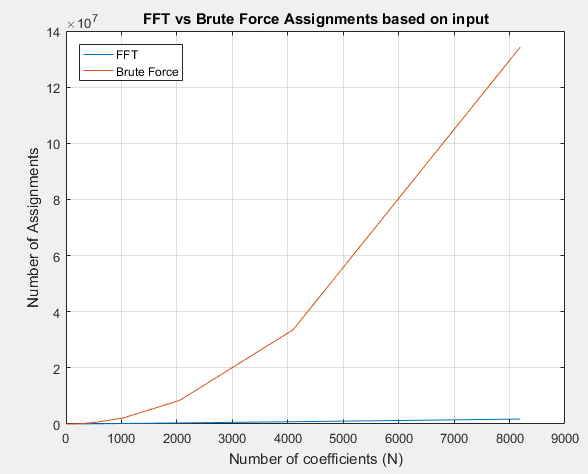
\includegraphics[scale=0.5]{images/BruteVSFFT_8192}}
            \caption{Number of Assignments. FFT vs Brute Force.}
            \label{fig:assign8192}
        \end{figure} 
        \begin{figure}[H]
            \centerline{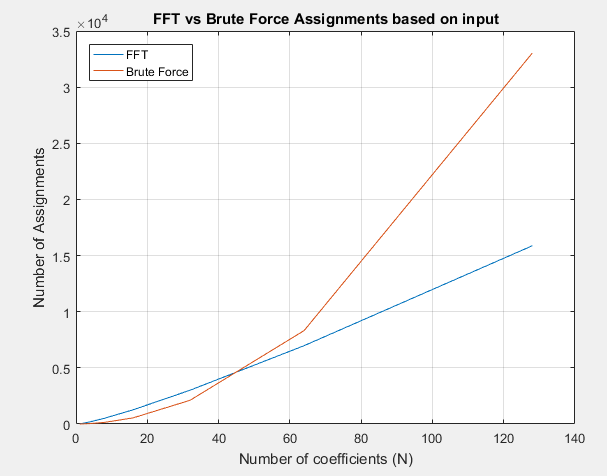
\includegraphics[scale=0.5]{images/BruteVSFFT_ZoomIn}}
            \caption{Number of Assignments. FFT vs Brute Force.}
            \label{fig:assignZoom}
        \end{figure}
        \section{Discussion}
        \indent\par{Brute Force performs better for smaller degree polynomials (i.e. $< 45$ terms). Fast Fourier transforms have an overhead, however it quickly overcomes its quadratic counterpart.}
        
        %%%%%%%%%%%%%%%%%%%%%%%%%%%%
        %%% INCLUDE BIBLIOGRAPHY %%%
        %%%%%%%%%%%%%%%%%%%%%%%%%%%%
        \bibliography{Report.bib}
        \bibliographystyle{ieeetr}

    \end{document}    